\documentclass{beamer}

\usepackage{../cppenv, ../recdefs}

\usepackage{drawstack}
\usepackage{fourier}

\usetheme{Berkeley}

\newcommand{\Highlight}{\makebox[0pt][l]{\color{pink}\rule[-4pt]{\textwidth}{11pt}}}

\title{Exception Safety and Exception Handling}
\author{GKxx}
\date{\today}

\AtBeginSubsection{
    \begin{frame}{Contents}
        \tableofcontents[currentsection, currentsubsection]
    \end{frame}
}

\begin{document}

\begin{frame}
    \maketitle
\end{frame}

\begin{frame}{Contents}
    \tableofcontents
\end{frame}

\section{Things Tend to Go Wrong}

\begin{frame}[fragile]{Input Failure}
    \begin{cpp}
    int num_of_people;
    std::cin >> num_of_people;
    \end{cpp}
    What happens when the input is not an integer?
\end{frame}

\begin{frame}[fragile]{\ttt{strcpy}}
    You are asked to write a \ttt{strcpy} function...
    \begin{cpp}
void strcpy(char *dest, const char *source) {
  while (*source)
    *dest++ = *source++;
  *dest = '\0';
}
    \end{cpp}
    \pause
    In reality, things may go wrong:
    \begin{itemize}
        \item Null pointers?
        \item Buffer overflow?
    \end{itemize}
    Detecting buffer overflow may not be easy.
\end{frame}

\begin{frame}[fragile]{Which is Better?}
    \begin{columns}
        \begin{column}{0.5\textwidth}
            1. Terminate the program on failure and report the error.
            \begin{cpp}
void strcpy(char *dest,
    const char *source) {
  if (!dest || !source) {
    std::cerr << "Invalid arguments for strcpy.\n";
    exit(1);
  }
  while (*source)
    *dest++ = *source++;
  *dest = '\0';
}
            \end{cpp}
        \end{column}
        \begin{column}{0.5\textwidth}
            2. Return false on failure:
            \begin{cpp}
bool strcpy(char *dest,
    const char *source) {
  if (!dest || !source)
    return false;
  while (*source)
    *dest++ = *source++;
  *dest = '\0';
  return true;
}
            \end{cpp}
        \end{column}
    \end{columns}
\end{frame}

\begin{frame}[fragile]{Which is Better?}
    \begin{columns}
        \begin{column}{0.5\textwidth}
            3. Be silent to errors.
            \begin{cpp}
void strcpy(char *dest,
    const char *source) {
  if (dest && source) {
    while (*source)
      *dest++ = *source++;
    *dest = '\0';
  }
}
            \end{cpp}
        \end{column}
        \begin{column}{0.5\textwidth}
            4. Use assertions.
            \begin{cpp}
void strcpy(char *dest,
    const char *source) {
  assert(dest != NULL);
  assert(source != NULL);
  while (*source)
    *dest++ = *source++;
  *dest = '\0';
}
            \end{cpp}
        \end{column}
    \end{columns}
    \url{https://blog.csdn.net/myan/article/details/1921}
\end{frame}

\section{Exception Handling}

\subsection{\ttt{throw}}

\begin{frame}[fragile]{Throwing an Exception}
    \begin{cpp}
void strcpy(char *dest, const char *source) {
  if (!dest || !source)
    throw std::invalid_argument("Null pointers passed to strcpy.");
  while (*source)
    *dest++ = *source++;
  *dest = '\0';
}
    \end{cpp}
\end{frame}

\begin{frame}{Standard Exceptions}
    \begin{center}
        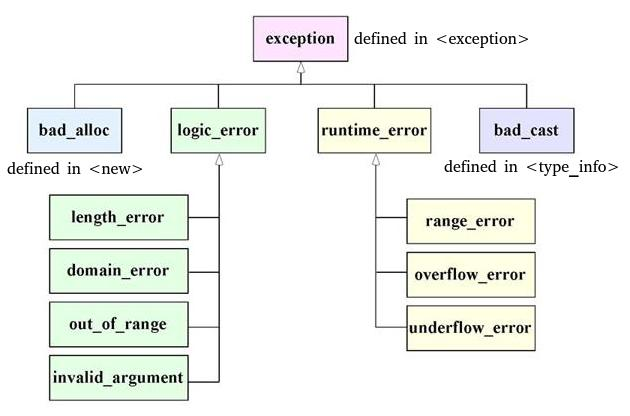
\includegraphics[width=0.9\textwidth]{img/ExceptionClasses.jpg}
    \end{center}
    \begin{itemize}
        \item \ttt{logic\_error}, \ttt{runtime\_error} and their subclasses are defined in \ttt{<stdexcept>}.
    \end{itemize}
\end{frame}

\begin{frame}{Standard Exceptions}
    \begin{itemize}
        \item The normal \bluett{new} and \bluett{new}\ttt{[]} operators throw \ttt{std::bad\_alloc} when running out of memory.
        \item \bluett{dynamic\_cast} for references throws \ttt{std::bad\_cast} when the casting fails.
        \begin{itemize}
            \item \bluett{dynamic\_cast} for pointers does not throw. It returns \bluett{nullptr} on failure.
        \end{itemize}
        \pause
        \item \ttt{std::system\_error} is thrown in many cases, especially in functions that interface with \blue{OS facilities}, e.g. the constructor of \ttt{std::thread}.
        \item \ttt{<chrono>} defines \ttt{std::nonexistent\_local\_time} and \ttt{std::ambiguous\_local\_time}.
    \end{itemize}
\end{frame}

\begin{frame}[fragile]{Standard Exceptions}
    \ttt{operator[]} for STL containers does not check boundaries, but \ttt{at()} does.
    \begin{cpp}
std::vector<int> v;
v.at(0) = 42; // Throws std::out_of_range.
v[0] = 42; // Does not throw, but probably causes a segmentation fault.
    \end{cpp}
    We will see that exceptions \bluett{throw}n could be \bluett{catch}-ed and handled.
\end{frame}

\begin{frame}[fragile]{Standard Exceptions}
    Let our \ttt{Array} do the same thing?
    \begin{cpp}
template <typename T>
class Array {
 public:
  const T &at(std::size_t n) const {
    if (n >= m_size)
      throw std::out_of_range("Array subscript out of range.");
    return m_data[n];
  }
  T &at(std::size_t n) {
    return const_cast<T &>(
      static_cast<const Array<T> *>(this)->at(n);
    ) // see Effective C++ Item 3
  }
  // ...
};
    \end{cpp}
\end{frame}

\begin{frame}[fragile]{Stack Unwinding}
    \begin{columns}
        \begin{column}{0.5\textwidth}
            \begin{cpp}
void func(int n) {
  int x = 42;
  int *p = new int[n];
  // ...
}
int main() {
  int size = 100;
  func(size);
  // ...
}
            \end{cpp}
        \end{column}
        \begin{column}{0.5\textwidth}
            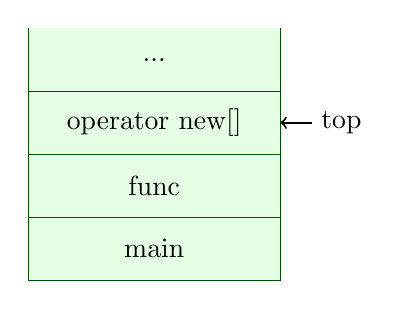
\begin{tikzpicture}[scale=0.8]
                \stacktop{}
                \cell{\bluett{operator new}\ttt{[]}}\cellptr{top}
                \cell{\ttt{func}}
                \cell{\ttt{main}}
            \end{tikzpicture}
        \end{column}
    \end{columns}
    Suppose \bluett{operator new}\ttt{[]} encounters shortage of memory...
\end{frame}

\begin{frame}[fragile]{Stack Unwinding}
    \begin{columns}
        \begin{column}{0.4\linewidth}
            \begin{lstlisting}[language = {[11]C++}, escapechar = \@]
@\onslide<4>{\Highlight}@void func(int n) {
@\onslide<3>{\Highlight}@  int x = 42;
@\onslide<1,2>{\Highlight}\onslide<1>{\danger}@int *p = new int[n];
  // ...
}
int main() {
@\onslide<6>{\Highlight}@  int size = 100;
@\onslide<5>{\Highlight}@  func(size);
  // ...
}
            \end{lstlisting}
        \end{column}
        \begin{column}{0.6\linewidth}
            \begin{enumerate}
                \onslide<1->\item \ttt{std::bad\_alloc} is raised in \bluett{operator new}\ttt{[]}.
                \onslide<2->\item Control flow returns to \ttt{func}.
                \onslide<3->\item \ttt{x} is destroyed.
                \onslide<4->\item \ttt{n} is destroyed.
                \onslide<5->\item Control flow returns to \ttt{main}.
                \onslide<6->\item \ttt{size} is destroyed.
            \end{enumerate}
        \end{column}
    \end{columns}
    \onslide<7->
    \begin{notice}
        Stack unwinding is only guaranteed to happen for \textbf{caught} exceptions. If an exception is not caught, whether the stack is unwound is \textbf{implementation-defined}.
    \end{notice}
\end{frame}

\subsection{\ttt{try}-\ttt{catch}}

\begin{frame}[fragile]{Catch an Exception}
    \begin{cpp}
void func(int n) {
  int x = 42;
  int *p = new int[n];
  // ...
}
int main() {
  try {
    int size = 100;
    func(size):
  } catch (const std::bad_alloc &e) {
    // deal with shortage of memory here.
  }
  // ...
}
    \end{cpp}
    \textit{More Effective C++} Item 13: Catch exceptions by reference.
\end{frame}

\begin{frame}[fragile]{\ttt{what}}
    The error message could be obtained via the `\ttt{what}' member function, which is \bluett{virtual}, \bluett{const} and \bluett{noexcept}.
    \begin{cpp}
void fun() {
  throw std::runtime_error("I love watermelons.");
}
int main() {
  try {
    fun();
  } catch (const std::runtime_error &re) {
    std::cout << re.what() << std::endl;
  }
}
    \end{cpp}
    Output:
    \begin{txt}
I love watermelons.
    \end{txt}
\end{frame}

\begin{frame}[fragile]{Catch an Exception}
    \begin{cpp}
void f(const std::vector<int> &v) {
  try {
    int i = 42;
    std::vector<int> copy = v;
    int x = copy.at(100);
    g(x);
  } catch (const std::bad_alloc &ba) {
    // deal with shortage of memory
  } catch (const std::out_of_range &oor) {
    // deal with illegal subscript '100'
  } catch (...) {
    // What else may happen? idk
    throw; // Throw the exception again.
  }
  std::cout << "returns.\n";
}
    \end{cpp}
\end{frame}

\newcommand{\commenter}[1]{\footnotesize\gray{#1}}

\begin{frame}[fragile]{Catch an Exception}
    Suppose \ttt{std::out\_of\_range} is raised.
    \begin{lstlisting}[language = {[11]C++}, escapechar = \@]
void f(const std::vector<int> &v) {
  try {
@\onslide<3>{\Highlight}@    int i = 42;@\onslide<3>{\quad\quad\quad\quad\commenter{`i' is destroyed}}@
@\onslide<2>{\Highlight}@    std::vector<int> copy = v;@\onslide<2>{\quad\commenter{`copy' is destroyed}}@
@\onslide<1>{\Highlight\danger}@  int x = copy.at(100);@\onslide<1>{\quad\quad\quad\commenter{throws \ttt{std::out\_of\_range}}}@
    g(x);
@\onslide<4>{\Highlight}@  } catch (const std::bad_alloc &ba) {@\onslide<4>{\quad\commenter{Not matched}}@
    // deal with shortage of memory
@\onslide<5>{\Highlight}@  } catch (const std::out_of_range &oor) {@\onslide<5>{\quad\commenter{Matched}}@
@\onslide<6>{\Highlight}@    // deal with illegal subscript '100'
  } catch (...) {
    // What else may happen? idk
    throw; // Throw the exception again.
  }
@\onslide<7>{\Highlight}@  std::cout << "returns\n";@\onslide<7>{\quad\commenter{Control flow continues here}}@
}
    \end{lstlisting}
\end{frame}

\begin{frame}[fragile]{Catch by Base Class}
    \bluett{operator new}\ttt{[]} raises \ttt{std::bad\_alloc} when out of memory.
    \begin{itemize}
        \item But if the array-new length is obviously invalid, an instance of \ttt{std::bad\_array\_new\_length} is raised.
        \begin{cpp}
new int[-1]; // negative size
new int[3]{2, 3, 4, 6, 8}; // too many initializers
new int[LONG_MAX][100]; // too large
        \end{cpp}
        \pause
        \item \bluett{catch }\ttt{(}\bluett{const }\ttt{std::bad\_alloc \&)} also catches it, because of \textbf{inheritance}:
        \begin{figure}[h]
            \centering
            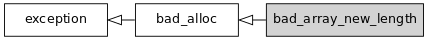
\includegraphics[scale=0.7]{img/bad_array_new_length-inheritance.png}
        \end{figure}
    \end{itemize}
\end{frame}

\begin{frame}[fragile]{Catch by Base Class}
    \begin{cpp}
try {
  do_something();
} catch (const std::runtime_error &re) {
  // deal with runtime_error
} catch (const std::exception &e) {
  // deal with other kinds of exceptions
} catch (...) {
  // deal with other things
}
    \end{cpp}
    \pause
    Note: Other things (e.g. a string) can also be \bluett{throw}n.
    \begin{cpp}
throw "I don\'t want to talk to you.";
    \end{cpp}
    In this case, these things are caught by \bluett{catch }\ttt{(...)}.
\end{frame}

\begin{frame}[fragile]{Catch by Base Class}
    \bluett{catch} clauses are examined one-by-one.
    \begin{cpp}
try {
  do_something();
} catch (const std::exception &e) {
  std::cout << "exception\n";
} catch (const std::runtime_error &re) {
  std::cout << "runtime_error\n";
} catch (...) {
  // deal with other things
}
    \end{cpp}
    If an instance of \ttt{std::runtime\_error} is thrown, it will be caught by ``\bluett{const }\ttt{std::exception \&}'' instead of ``\bluett{const }\ttt{std::runtime\_error \&}'' in this case.
\end{frame}

\begin{frame}[fragile]{Stack Unwinding}
    \begin{lstlisting}[language = {[11]C++}, escapechar = \@]
void fun() {
@\onslide<3>{\Highlight}@  int i = 42;@\onslide<3>{\quad\quad\commenter{`i' is destroyed}}@
@\onslide<2>{\Highlight}@  std::vector<int> v;@\onslide<2>{\quad\commenter{`v' is destroyed}}@
@\onslide<1>{\Highlight\danger}@v.at(i) = 10;@\onslide<1>{\quad\quad\commenter{throws std::out\_of\_range}}@
}
int main() {
  try {
@\onslide<5>{\Highlight}@    std::string str("Hello");@\onslide<5>{\quad\commenter{`str' is destroyed}}@
@\onslide<4>{\Highlight}@    fun();@\onslide<4>{\quad\quad\commenter{Control flow returns here}}@
@\onslide<6>{\Highlight}@  } catch (...) {}@\onslide<6>{\quad\commenter{The exception is caught.}}@
}
    \end{lstlisting}
\end{frame}

\begin{frame}[fragile]{Notes}
    \begin{itemize}
        \item The \bluett{try} block and \bluett{catch} blocks are independent scopes. Objects declared in the \bluett{try} block cannot be used in \bluett{catch} blocks.
        \item When an exception occurs, local objects in the \bluett{try} block are destroyed before the exception is caught.
        \item Stack unwinding is only guaranteed to happen for \textbf{caught} exceptions.
        \item If an exception is thrown and not caught, `\ttt{std::terminate}' will be called to terminate the program. (defined in \ttt{<exception>})
    \end{itemize}
\end{frame}

\begin{frame}[fragile]{\ttt{try}-\ttt{catch} for Constructors}
    \begin{cpp}
template <typename T>
class Array {
 public:
  Array(std::size_t n)
      try : m_size(n), m_data(new T[n]{}) {}
  catch (const std::bad_alloc &ba) {
    std::cerr << "No enough memory.\n";
    throw;
  }
};
    \end{cpp}
    Notes:
    \begin{itemize}
        \item Exceptions raised both in \blue{constructor initializer list} and \blue{function body} can be caught.
        \item Non-static data members cannot be referred to in such \bluett{catch} blocks. \red{(Why?)}
    \end{itemize}
\end{frame}

\subsection{User-defined Exception Classes}

\begin{frame}[fragile]{User-defined Exceptions}
    \begin{cpp}
class Wrong_answer : public std::logic_error {
 public:
  Wrong_answer(std::size_t line_no)
      : std::logic_error("Wrong answer on line "
          + std::to_string(line_no)) {}
};
#define assert(X)                          \
  { if (!(X)) throw Wrong_answer(__LINE__); }
int main() {
  int a = rand(), b = rand();
  int ans = add(a, b);
  assert(ans == a + b);
  return 0;
}
    \end{cpp}
\end{frame}

\section{Exception Safety}

\subsection{Exception-safety Guarantees}

\begin{frame}{Exception-safety Guarantees}
    Exception-safe functions offer one of three guarantees:
    \begin{itemize}
        \item \textbf{Nothrow guarantee}: Promise never to throw exceptions.
        \item \textbf{Strong guarantee}: Promise that if an exception is thrown, the state of the program is unchanged (as if the function had not been called).
        \item \textbf{Weak guarantee} (basic guarantee): Promise that if an exception is thrown, everything in the program remains in a valid state.
        \begin{itemize}
            \item No objects or data structures become corrupted.
            \item All class invariants are satisfied.
        \end{itemize}
    \end{itemize}
    \textit{Effective C++} Item 29: Strive for exception-safe code.
\end{frame}

\begin{frame}{Exception-safety Guarantees}
    \textit{Effective C++} Item 29:
    \begin{quotation}
        A software system is \textbf{either exception-safe or it's not}. There's no such thing as a partially exception-safe system. If a system has \textbf{even a single function} that's not exception-safe, the system as a whole is not exception-safe.
    \end{quotation}
    \pause
    \begin{quotation}
        A function can usually offer a guarantee no stronger than the \textbf{weakest} guarantee of the functions it calls.
    \end{quotation}
\end{frame}

\subsection{Exception Specifications}

\begin{frame}[fragile]{\ttt{noexcept} vs \ttt{throw()}}
    Before C++11, a function may declare in advance what exception it may throw.
    \begin{cpp}
void *operator new(std::size_t size) throw(std::bad_alloc);
    \end{cpp}
    \pause
    To declare that a function does not throw exceptions:
    \begin{cpp}
int add(int a, int b) throw() {
  return a + b;
}
    \end{cpp}
\end{frame}

\begin{frame}[fragile]{\ttt{noexcept} vs \ttt{throw()}}
    People came to realize that it is \textbf{whether the function throws exceptions or not} that really matters.\par
    \pause
    Since C++11, declare \bluett{noexcept} for non-throwing functions.
    \begin{cpp}
template <typename T>
void swap(Array<T> &a, Array<T> &b) noexcept {
  a.swap(b);
}
    \end{cpp}
    \pause
    The \ttt{throw()} specifiers have been deprecated and removed in modern C++.
\end{frame}

\begin{frame}{\ttt{noexcept}}
    The \bluett{noexcept} specifier makes it possible for more optimization.
    \begin{itemize}
        \item When an exception is thrown inside a \bluett{noexcept} function, the stack is \textit{possibly} unwound.
        \begin{itemize}
            \item Compilers need not keep the runtime stack in an unwindable state.
        \end{itemize}
        \item Certain functions must be \bluett{noexcept} so that they can be called by standard library functions.
        \begin{itemize}
            \item Move constructors and move assignment operators.
        \end{itemize}
    \end{itemize}
\end{frame}

\begin{frame}{\ttt{noexcept}}
    \bluett{noexcept} is not checked in compile-time. A \bluett{noexcpet} function may still
    \begin{itemize}
        \item call functions that are not \bluett{noexcept}, or
        \item throw exceptions under certain circumstances.
    \end{itemize}
\end{frame}

\begin{frame}[fragile]{Arguments to \ttt{noexcept}}
    \bluett{noexcept} may take one argument that is a \blue{constant expression} and is convertible to \bluett{bool}.
    \begin{cpp}
// noexcept iff T is nothrow-copy-constructible.
template <typename T>
void fun() noexcept(
    std::is_nothrow_copy_constructible<T>::value) {
  // ...
}
    \end{cpp}
    \bluett{noexcept} is equivalent to \bluett{noexcept}\ttt{(}\bluett{true}\ttt{)}.
\end{frame}

\begin{frame}[fragile]{The \ttt{noexcept} Operator}
    \bluett{noexcept} can also work as an operator, which returns a \bluett{bool} value indicating whether an expression throws exceptions.
    \begin{cpp}
template <typename T>
class Box {
  T thing;
 public:
  void swap(Box<T> &other)
      noexcept(noexcept(std::swap(thing, other.thing)))
  {
    std::swap(thing, other.thing);
  }
};
    \end{cpp}
\end{frame}

\subsection{Example: Copy Control}

\begin{frame}[fragile]{Which Exception-safety Guarantee?}
    \begin{cpp}
class Array {
  int *m_data;
  std::size_t m_size;

 public:
  Array &operator=(const Array &other) {
    if (this != &other) {
      delete[] m_data;
      m_data = new int[other.m_size];
      std::copy(other.m_data,
                other.m_data + other.m_size, m_data);
      m_size = other.m_size;
    }
    return *this;
  }
};
    \end{cpp}
    \pause
    \textbf{It does not offer even the basic guarantee.}
\end{frame}

\begin{frame}[fragile]{Which Exception-safety Guarantee?}
    \begin{cpp}
class Array {
 public:
  Array &operator=(const Array &other) {
    auto new_data = new int[other.m_size];
    std::copy(other.m_data,
              other.m_data + other.m_size, new_data);
    delete[] m_data;
    m_data = new_data;
    m_size = other.m_size;
    return *this;
  }
};
    \end{cpp}
    \pause
    \textbf{Strong guarantee.}
\end{frame}

\begin{frame}[fragile]{Which Exception-safety Guarantee?}
    \begin{cpp}
class Array {
 public:
  Array &operator=(const Array &other) {
    m_size = other.m_size;
    auto new_data = new int[m_size];
    std::copy(other.m_data,
              other.m_data + m_size, new_data);
    delete[] m_data;
    m_data = new_data;
    return *this;
  }
};
    \end{cpp}
    \pause
    \textbf{No exception-safety guarantee.}
\end{frame}

\begin{frame}[fragile]{Which Exception-safety Guarantee?}
    \begin{cpp}
class Array {
 public:
  void swap(Array &other) noexcept {
    using std::swap;
    swap(m_size, other.m_size);
    swap(m_data, other.m_data);
  }
  Array &operator=(const Array &other) {
    Array(other).swap(*this);
    return *this;
  }
};
    \end{cpp}
    \pause
    \textbf{Strong guarantee.}
\end{frame}

\begin{frame}[fragile]{Which Part may Throw?}
    \begin{lstlisting}[language = {[11]C++}, escapechar = \@]
// For simplicity, assume T is default-constructible and copy-assignable.
@\redtt{template <typename T>}@
class Array {
  @\redtt{T *}@m_data;
  std::size_t m_size;

 public:
  Array(const Array &other)
      : m_data(new T[other.m_size]),
        m_size(other.m_size) {
    std::copy(other.m_data,
              other.m_data + other.m_size, m_data);
  }
};
    \end{lstlisting}
\end{frame}

\begin{frame}[fragile]{Which Exception-safety Guarantee?}
    \begin{cpp}
template <typename T>
class Array {
 public:
  Array(const Array &other)
      : m_data(new T[other.m_size]),
        m_size(other.m_size) {
    std::copy(other.m_data,
              other.m_data + other.m_size, m_data);
  }
};
    \end{cpp}
    \pause
    \textbf{No guarantee.} If an exception occurs when copying, \ttt{m\_size} and \ttt{m\_data} will be destroyed, resulting in \textbf{memory leak}.
\end{frame}

\begin{frame}[fragile]{Make it Exception-safe}
    \begin{lstlisting}[language = {[11]C++}, escapechar = \@]
template <typename T>
class Array {
 public:
  Array(const Array &other)
      : m_data(new T[other.m_size]),
        m_size(other.m_size) {
    try {
      std::copy(other.m_data,
                other.m_data + other.m_size, m_data);
    } catch (...) {
      delete[] m_data; // Avoid memory leak
      @\redtt{throw;}@ // Let the caller know it!
    }
  }
};
    \end{lstlisting}
\end{frame}

\begin{frame}[fragile]{Which Exception-safety Guarantee?}
    \begin{cpp}
template <typename T>
class Array {
 public:
  Array &operator=(const Array &other) {
    auto new_data = new T[other.m_size];
    std::copy(other.m_data,
              other.m_data + other.m_size, new_data);
    delete[] m_data;
    m_data = new_data;
    m_size = other.m_size;
    return *this;
  }
};
    \end{cpp}
    \pause
    \textbf{No guarantee.}
\end{frame}

\begin{frame}[fragile]{Make it Exception-safe}
    \begin{lstlisting}[language = {[11]C++}, escapechar = \@]
template <typename T>
class Array {
 public:
  Array &operator=(const Array &other) {
    auto new_data = new T[other.m_size];
    try {
      std::copy(other.m_data,
                other.m_data + other.m_size, new_data);
    } catch (...) {
      delete[] new_data;
      throw;
    }
    delete[] m_data;
    m_data = new_data;
    m_size = other.m_size;
    return *this;
  }
};
    \end{lstlisting}
\end{frame}

\begin{frame}[fragile]{Which Exception-safety Guarantee?}
    \begin{cpp}
template <typename T>
class Array {
 public:
  void swap(Array &other) noexcept {
    using std::swap;
    swap(m_size, other.m_size);
    swap(m_data, other.m_data);
  }
  Array &operator=(const Array &other) {
    Array(other).swap(*this);
    return *this;
  }
};
    \end{cpp}
    \pause
    \textbf{Strong guarantee.}
\end{frame}

\end{document}